% Standalone TikZ figure: Two-Stage vs One-Stage Detector Architecture Comparison
% For Chapter 2: Background and Theoretical Foundations
\documentclass[tikz,border=10pt]{standalone}
\usepackage{tikz}
\usetikzlibrary{arrows.meta, positioning, shapes.geometric, fit, backgrounds, calc, decorations.pathreplacing}

\begin{document}
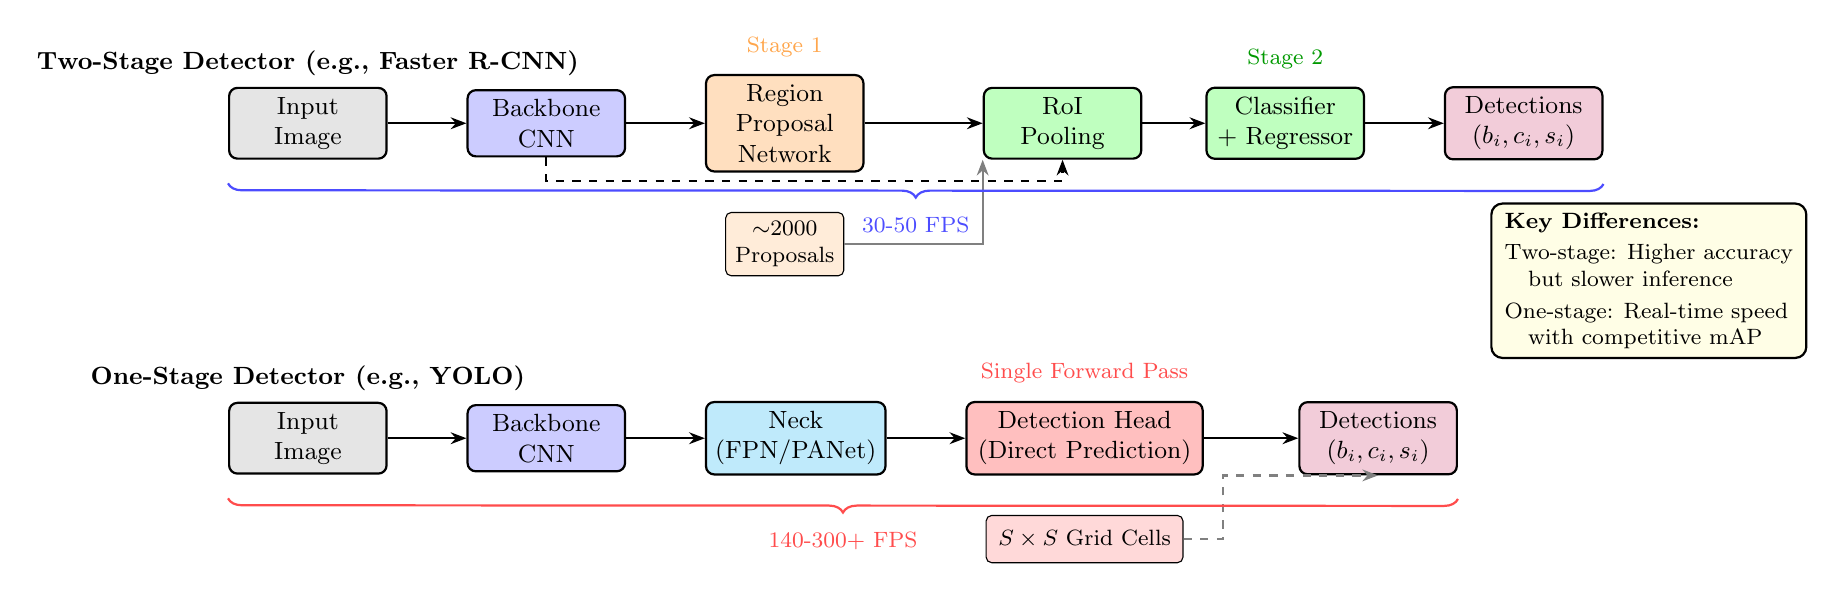
\begin{tikzpicture}[
    node distance=0.8cm and 1.2cm,
    every node/.style={font=\small},
    box/.style={rectangle, draw, thick, minimum width=2cm, minimum height=0.8cm, align=center, rounded corners=3pt},
    smallbox/.style={rectangle, draw, minimum width=1.5cm, minimum height=0.6cm, align=center, rounded corners=2pt, font=\footnotesize},
    arrow/.style={-{Stealth[length=2mm]}, thick},
    label/.style={font=\footnotesize},
    title/.style={font=\bfseries\small}
]

% ============ TWO-STAGE DETECTOR (TOP) ============
\node[title] at (0, 0.5) {Two-Stage Detector (e.g., Faster R-CNN)};

% Input image
\node[box, fill=gray!20, below=0.3cm of {(0,0.5)}] (input1) {Input\\Image};

% Backbone
\node[box, fill=blue!20, right=1cm of input1] (backbone1) {Backbone\\CNN};

% Stage 1: RPN
\node[box, fill=orange!25, right=1cm of backbone1] (rpn) {Region\\Proposal\\Network};

% Proposals
\node[smallbox, fill=orange!15, below=0.5cm of rpn] (proposals) {$\sim$2000\\Proposals};

% Stage 2: Classification
\node[box, fill=green!25, right=1.5cm of rpn] (roi) {RoI\\Pooling};
\node[box, fill=green!25, right=0.8cm of roi] (classifier) {Classifier\\+ Regressor};

% Output
\node[box, fill=purple!20, right=1cm of classifier] (output1) {Detections\\$(b_i, c_i, s_i)$};

% Arrows for two-stage
\draw[arrow] (input1) -- (backbone1);
\draw[arrow] (backbone1) -- (rpn);
\draw[arrow] (rpn) -- (roi);
\draw[arrow] (roi) -- (classifier);
\draw[arrow] (classifier) -- (output1);
\draw[arrow, dashed] (backbone1.south) -- ++(0,-0.3) -| (roi.south);
\draw[arrow, gray] (proposals.east) -| (roi.south west);

% Stage labels
\node[label, above=0.1cm of rpn, text=orange!70] {Stage 1};
\node[label, above=0.1cm of classifier, text=green!60!black] {Stage 2};

% ============ ONE-STAGE DETECTOR (BOTTOM) ============
\node[title] at (0, -3.5) {One-Stage Detector (e.g., YOLO)};

% Input image
\node[box, fill=gray!20, below=0.3cm of {(0,-3.5)}] (input2) {Input\\Image};

% Backbone
\node[box, fill=blue!20, right=1cm of input2] (backbone2) {Backbone\\CNN};

% Neck (Feature Pyramid)
\node[box, fill=cyan!25, right=1cm of backbone2] (neck) {Neck\\(FPN/PANet)};

% Detection Head - single unified
\node[box, fill=red!25, right=1cm of neck, minimum width=3cm] (head) {Detection Head\\(Direct Prediction)};

% Grid illustration
\node[smallbox, fill=red!15, below=0.5cm of head, minimum width=2.5cm] (grid) {$S \times S$ Grid Cells};

% Output
\node[box, fill=purple!20, right=1.2cm of head] (output2) {Detections\\$(b_i, c_i, s_i)$};

% Arrows for one-stage
\draw[arrow] (input2) -- (backbone2);
\draw[arrow] (backbone2) -- (neck);
\draw[arrow] (neck) -- (head);
\draw[arrow] (head) -- (output2);
\draw[arrow, gray, dashed] (grid.east) -- ++(0.5,0) |- (output2.south);

% Single pass annotation
\node[label, above=0.1cm of head, text=red!70] {Single Forward Pass};

% ============ COMPARISON ANNOTATIONS ============
% Speed comparison
\draw[decorate, decoration={brace, amplitude=5pt, mirror}, thick, blue!70]
    ([yshift=-0.3cm]input1.south west) -- ([yshift=-0.3cm]output1.south east)
    node[midway, below=0.3cm, font=\footnotesize, text=blue!70] {30-50 FPS};

\draw[decorate, decoration={brace, amplitude=5pt, mirror}, thick, red!70]
    ([yshift=-0.3cm]input2.south west) -- ([yshift=-0.3cm]output2.south east)
    node[midway, below=0.3cm, font=\footnotesize, text=red!70] {140-300+ FPS};

% Key differences box
\node[draw, thick, rounded corners, fill=yellow!10,
      minimum width=4cm, align=left, font=\footnotesize,
      right=0.5cm of {$(output1)!0.5!(output2)$}] (diff) {
    \textbf{Key Differences:}\\[2pt]
    Two-stage: Higher accuracy\\
    \hspace{1em}but slower inference\\[2pt]
    One-stage: Real-time speed\\
    \hspace{1em}with competitive mAP
};

\end{tikzpicture}
\end{document}
